\chapter{Medical Dataset}

\section{Overview}

Dane pochodzą z Duke University. Są to zdjęcia z rezonansu magnetycznego głowy wraz z zaznaczonymi obszarami zmian nowotworowych. Obrazy są rozmiaru 256x256x3. Pierwszy kanał jest zdjęciem wykonanym przed wprowadzeniem kontrastu, drugi w trakcie, a trzeci po. Maski mają rozmiar 256x256, a każdy piksel ma wartość 0 albo 255 (255 oznacza komórkę nowotworową). Na rysunku \ref{fig:medical_description} pokazane są osobne kanały oraz maska.

\begin{figure}[h!]
    \centering
    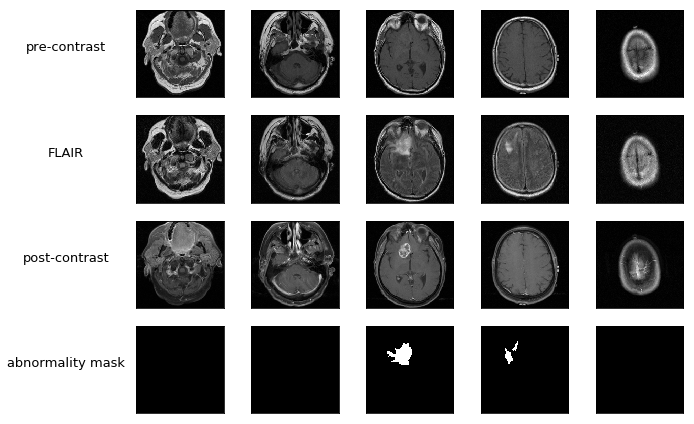
\includegraphics[width=0.8\textwidth]{images/medical_description}
    \caption{}
    \label{fig:medical_description}
\end{figure}

Dane pogrupowane są dla 110 pacjentów. Zestaw dla jednego z nich znajduje się na rysunku \ref{fig:medical_sample}. Łącznie znajduje się 3929 par obrazów, z czego w 1373 jest przynajmniej jedna komórka nowotworowa ($\sim$34.95\%). Natomiast w całym zbiorze piksele oznaczające zmiany nowotworowe stanowią jedynie $\sim$1.02988\% wszystkich pikseli. Przy tak znaczącej dysproporcji ciężko liczyć na rzetelne podejście supervised, dlatego będę chciał spróbować podejścia unsupervised. Założeniem wykorzystania VAE będzie patrzenie na koszty. Hipotezą jest to, że obrazki z rakiem, czyli takie mało prawdopodobne będą zauważalne w rozkładzie i rekonstrukcji.

\begin{figure}[h!]
    \centering
    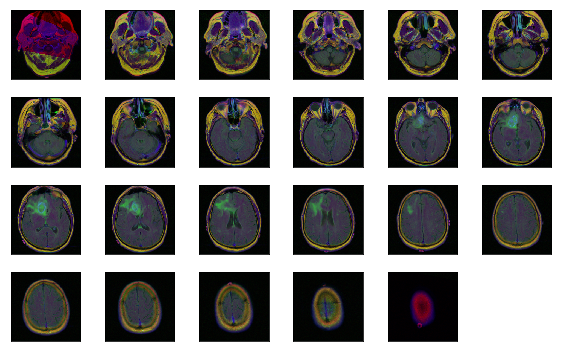
\includegraphics[width=0.8\textwidth]{images/medical_sample}
    \caption{}
    \label{fig:medical_sample}
\end{figure}

Pacjenci zostali podzieleni na 2 zbiory: treningowy (70\%), testowy (30\%). Obrazki oznaczające komórki rakowe będę nazywał pozytywnymi, a tez bez negatywnymi.

\section{Patches}

Rekonstrukcje nie chcemy robić od razu z całego obrazku, a jedynie z niewielkich wycinków. Rozmiar wycinków ustalę na podstawie wyników osiąganych przez modele supervised, tj. regresja liniowa, małe cnn (mnist), cnn (cifar10). Będę testował rozmiary 16, 22, 28, 32, 48, 64. 

Na obrazku \ref{fig:supervised_patches} widać wyniki dla poszczególnych modeli i rozmiarów. Patrzymy na 2 wartości true positive rate i true negative rate. Najepszy przypadek jest w takim razie w punkcie (1, 1). Obrazek (d) prezentuje średnie wyniki dla każdego z rozmiaru. Przy takim liczeniu najlepsze wyniki wyszły dla rozmiarów odpowiednio 16 i 22. W dalszych eksperymentach będę korzystał z pachy o rozmiarze 22 ze względu na troche wieksze pole obserwacji.

\begin{figure}[h!]
  \centering
  \begin{subfigure}[b]{0.45\linewidth}
    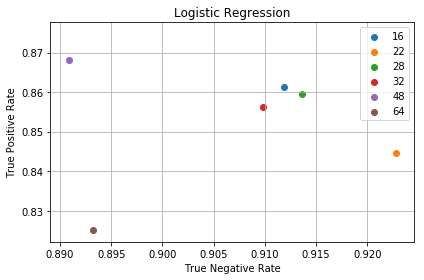
\includegraphics[width=\linewidth]{images/logreg_patch}
    \caption{Coffee.}
  \end{subfigure}
  \begin{subfigure}[b]{0.45\linewidth}
    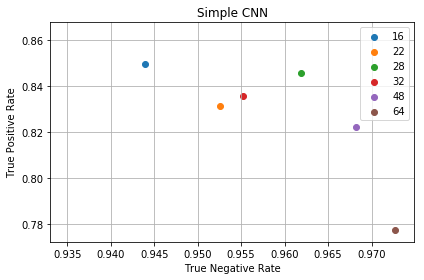
\includegraphics[width=\linewidth]{images/cnn_patch}
    \caption{More coffee.}
  \end{subfigure}
  \begin{subfigure}[b]{0.45\linewidth}
    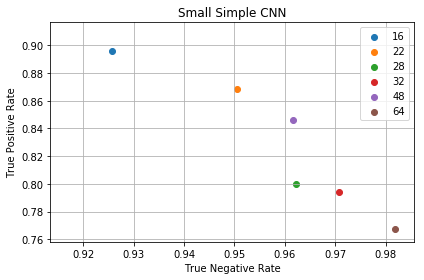
\includegraphics[width=\linewidth]{images/smallcnn_patch}
    \caption{More coffee.}
  \end{subfigure}
  \begin{subfigure}[b]{0.45\linewidth}
    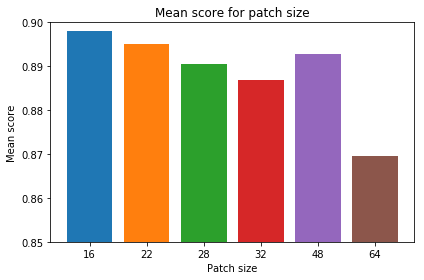
\includegraphics[width=\linewidth]{images/patch_score}
    \caption{More coffee.}
  \end{subfigure}
  \caption{The same cup of coffee. Two times.}
  \label{fig:supervised_patches}
\end{figure}
\todo{Uzupełnić podpisy}

\section{Preprocessing}

Na obrazku \ref{fig:pixel_sums} przedstawiony jest histogram zsumowanych wartości pikseli dla każdego patchu rozmiaru 22 z podziałem na klasy. Minimalna wartość sumy dla klasy pozytywnej wynosi $56.5$. Oznacza to, że ze zbioru treningowego można usunąć obrazki o mniejszej sumie, gdyż automatycznie są to negatywne obrazki. Usunięcie obrazków o wartości mniejszej niż 42 zmniejszy dane o $45.5\%$ i usunięcie trywialnych przypadków czyli prawie całych czarnych obrazków.

\begin{figure}[h!]
    \centering
    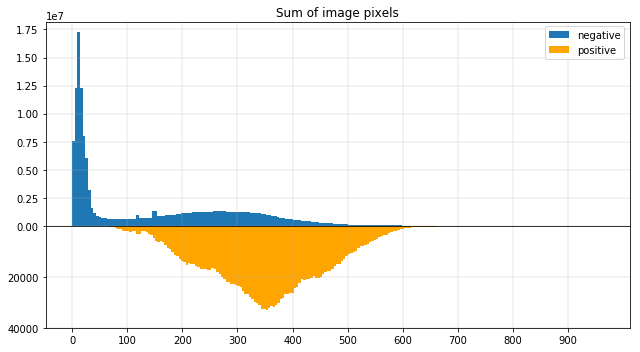
\includegraphics[width=0.7\textwidth]{images/pixel_sums}
    \caption{}
    \label{fig:pixel_sums}
\end{figure}

\section{Normalizations}

\todo[inline]{Może LIME?}

\todo[inline]{Rozważyć normalizacje: histogramowa, tylko środkowy kanał}
